\documentclass[
% opciók nélkül: egyoldalas nyomtatás, elektronikus verzió
% twoside,     % kétoldalas nyomtatás
% tocnopagenum,% oldalszámozás a tartalomjegyzék után kezdődik
]{thesis-ekf}
\usepackage[T1]{fontenc}
\PassOptionsToPackage{defaults=hu-min}{magyar.ldf}
\usepackage[magyar]{babel}
\usepackage{mathtools,amssymb,amsthm,pdfpages}
\footnotestyle{rule=fourth}

\newtheorem{tetel}{Tétel}[chapter]
\theoremstyle{definition}
\newtheorem{definicio}[tetel]{Definíció}
\theoremstyle{remark}
\newtheorem{megjegyzes}[tetel]{Megjegyzés}

\begin{document}
\institute{Matematikai és Informatikai Intézet}
\title{Jelenlét követő alkalmazás fejlesztése}
\author{Györkis Tamás\\Programtervező informatikus BSc}
\supervisor{Dr. Király Roland\\Egyetemi docens}
\city{Eger}
\date{2024}
\maketitle
\tableofcontents

\chapter*{Bevezetés}
\addcontentsline{toc}{chapter}{Bevezetés}
Amikor szakdolgozati témaválasztás előtt álltam, sokat gondolkoztam a témán. Mindenképpen egy olyan alkalmazást szerettem volna elkészíteni, mely ténylegesen hasznos is lehet. Egyetemi éveim alatt demonstrátorként tanítottam több féléven át az egyetemen, és innen jött a felismerés, hogy jó lenne, ha a hallgatók jelenlétét, hiányzásait ne táblázatokban kelljen vezetni, hanem egy külön eszköz legyen rá készítve. Innen származik az alkalmazás ötlete.

A megvalósítás során törekedtem arra, hogy egy jól átlátható, ergonomikus weboldalt készítsek, amit -- esetleges kisebb módosításokkal -- ne csak egyetemi környezetben lehessen használni. Ezekből kifolyólag egy webalkalmazást készítettem, mivel ezt a legegyszerűbb elérni, hiszen csak egy webböngésző szükséges hozzá. A tanulók és tanárok által használt oldalak reszponzívan lettek elkészítve, ezáltal biztosítva, hogy mobiltelefonon is használni lehessen. Illetve az alkalmazás PWA funkciókkal rendelkezik, aminek jelentőségére később térek ki, de előjáróban annyit érdemes megemlíteni róla, hogy lehetővé teszi a weboldal alkalmazásként való telepítését számítógép és telefon esetén is, ezáltal egy rendes alkalmazás érzését keltve.

A megvalósításhoz a Laravel keretrendszert használtam, mely egy PHP alapú, MVC keretrendszer, amivel tanulmányaim során találkoztam, és egyből megkedveltem. Nem titkolt célom a szakdolgozatommal, hogy bemutassam, hogy a mai, JavaScript preferált világban, továbbra is lehetséges modern, a mai kort kielégítő weboldalt készíteni PHP segítségével, amihez különböző csomagokat alkalmaztam, amiknek működését, illetve egymással való működését a későbbiekben fogom kifejteni.

\chapter{Alkalmazás bemutatása}
\section{Adatbázis}

\Aref{database} ábrán látható az alkalmazás által használt adatbázis, egyed-kapcsolat diagrammal ábrázolva, melyről szeretnék néhány szót ejteni.

\begin{figure}[ht!]
	\centering
	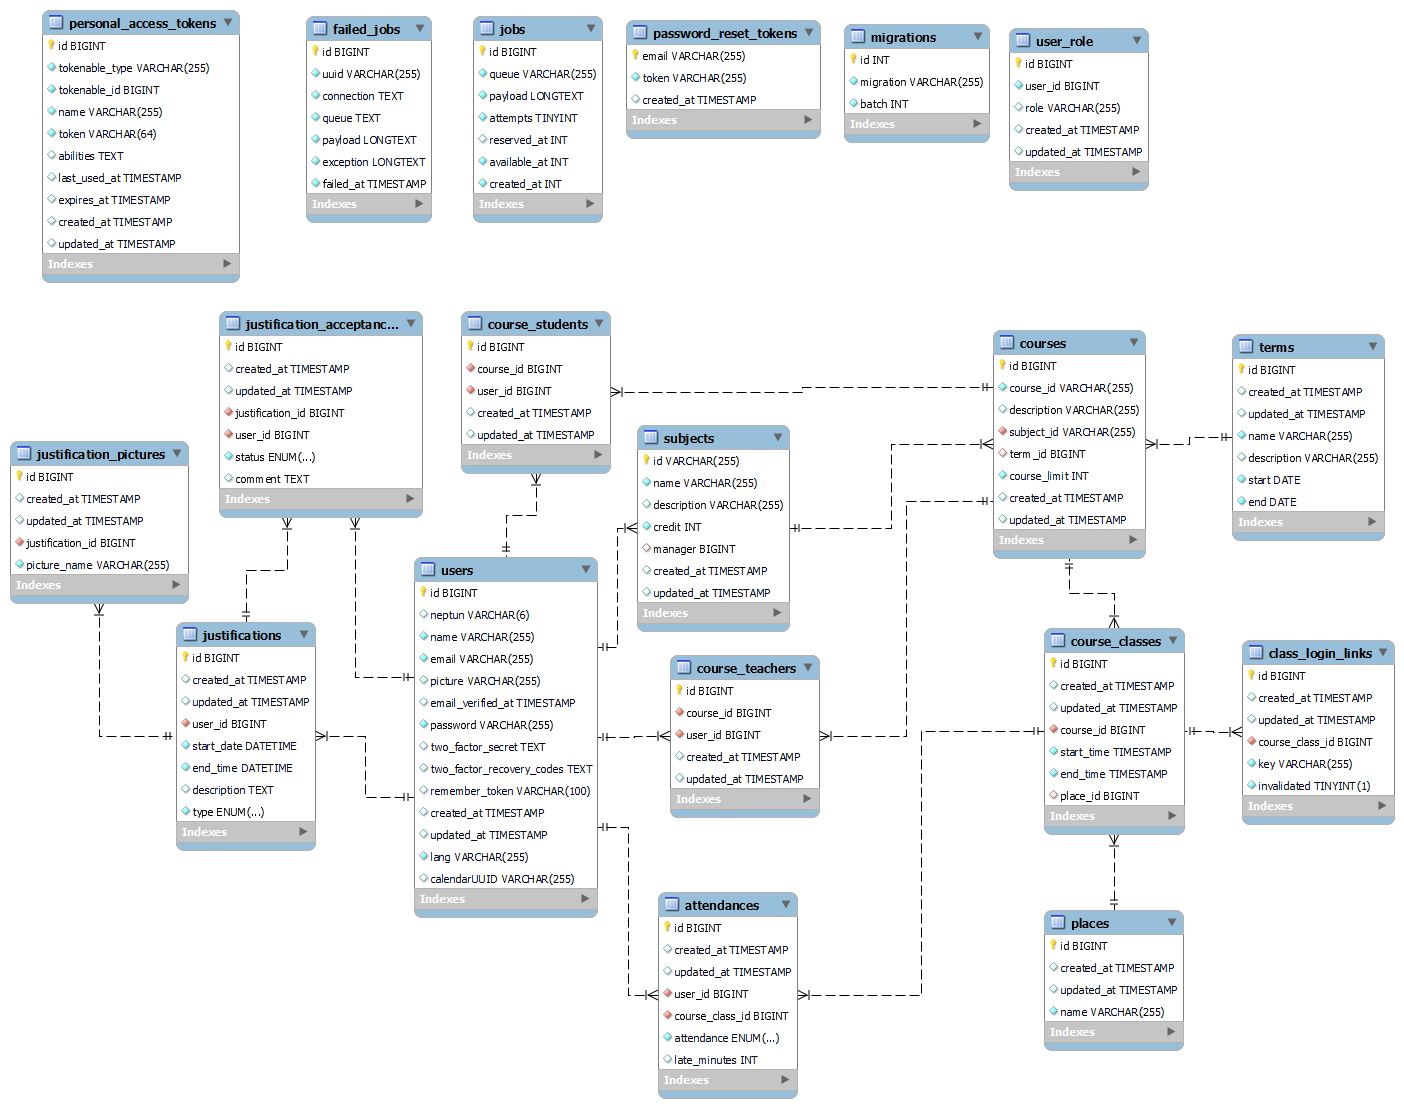
\includegraphics[width=15cm]{../pictures/db.png}
	\caption{Az alkalmazás által használt adatbázis.}
	\label{database}
\end{figure}

\begin{itemize}
	\item \emph{users}: ez a tábla tárolja a felhasználók adatait. Minden felhasználóról tárolunk egy azonosítót, egy Neptun kódot, nevet, email címet, egy titkosított jelszót, egy profilképet, a felhasználó által használt nyelvet, illetve egy UUID-t, azaz egy egyedi azonosítót, amit az órarend exportálásához lehet használni, erről később. Az azonosító oszlopra azért van szükség, mivel az alkalmazás fel van készítve arra, hogy Neptun kód nélkül rendelkező felhasználókat is tudjon kezelni.
	\item \emph{terms, places}: a félévek és termek (helyek) tárolására szolgáló táblák.
	\item \emph{subjects, courses, course\_classe, class\_login\_links}: ezen táblák tárolják a tantárgyakat (amik többek között rendelkeznek egy azonosítóval, névvel, leírással, kreditértékkel, és egy tantárgyfelelőssel), a tantárgyakhoz tartozó kurzusokat (amihez tárolok egy azonosítót, ami minden esetben egyedi, egy kurzus azonosítót, ami minden félév és tantárgy esetében kell egyedinek lennie, tartozik hozzá egy félév, illetve egy létszám limit), illetve kurzusokhoz pedig órák (amiknek van egy kezdete, vége, illetve egy terem, ahol tartják). Az utolsó tábla pedig az órákhoz tartozó bejelentkező linkeket tartalmazza, ennek jelentőségéről kicsit később.
	\item  \emph{attendances}: itt tárolom az egyes kurzusok résztvevőinek az órai jelenléteit, melyek lehetnek: nincs kitöltve, jelen, késés (mely esetben percben lehet tárolni a mértékét), hiányzás, igazolt hiányzás.
	\item \emph{justification, justification\_acceptances, justification\_pictures}: ezek a táblák tárolják az igazolásokat, az igazoláshoz tartozó feltöltött képeket, illetve az igazolásban érintett tanárok válaszát, hogy elfogadják-e ó, vagy sem.
	\item Az egyéb, nem említett táblák inkább kapcsolótábla funkciót töltenek be, vagy a keretrendszernek vannak rá szükségei. Például a \emph{jobs} tábla a háttérben végrehajtandó feladatokat (job) tartalmazza.
\end{itemize}

Itt érdemes még megemlíteni, hogy a fejlesztés során a MySQL nevezetű, relációs adatbázist használtam, viszont a Laravel keretrendszerből adódóan sok más típusú adatbázis szoftverrel használható az alkalmazás, mivel a táblák felépítése a keretrendszerben van elkészítve.

\section{Általános funkciók, információk}

Az alkalmazás elérhető a \url{https://szakdolgozat.ddns.net} címen, ahol ki lehet próbálni az alkalmazást. Pár alapértelmezett felhasználó elérhető:
\begin{itemize}
	\item Szuper adminisztrátor:
	\begin{itemize}
		\item Felhasználónév: \emph{SADMIN}
		\item Jelszó: \emph{superadmin}
	\end{itemize}
	\item Adminisztrátor:
	\begin{itemize}
		\item Felhasználónév: \emph{ADMIN0}
		\item Jelszó: \emph{admin}
	\end{itemize}
	\item Tanár:
	\begin{itemize}
		\item Felhasználónév: \emph{TEACHE}
		\item Jelszó: \emph{teacher}
	\end{itemize}
	\item Hallgató:
	\begin{itemize}
		\item Felhasználónév: \emph{STUDEN}
		\item Jelszó: \emph{student}
	\end{itemize}
\end{itemize}

\subsection{Felhasználók}



\section{Adminisztrátori nézet, funkciók}
\section{Tanári nézet, funkciók}
\section{Hallgatói nézet, funkciók}

\chapter{Felhasznált technológiák, csomagok}

\section{Laravel}
\subsection{Keretrendszer alapjai}
\subsection{MVC architektúra}
\subsection{Eloquent ORM}
\subsection{Blade templating engine}
\subsection{Laravel Fortify}
\subsection{Események, queue}
\subsection{Email küldés}

\section{Tailwind}
\subsection{DaisyUI}

\section{LiveWire}
\subsection{Ismertető, a csomag működése}
\subsection{LiveWire és SPA}
\subsection{Komponensek és data binding}
\subsection{Események, lapozás}
\subsection{Alpine.js: LiveWire és JavaScript kapcsolata}
\subsection{WireToast: LiveWire alapú értesítések}

\section{Websocket és Pusher szerviz}
\subsection{Websocket jelentősége}
\subsection{Pusher}
\subsection{Websocket integrálása a keretrendszerbe}
\subsection{Csatornák, események létrehozása}
\subsection{Események fogadása JavaScript, LiveWire esetén}

\section{QR-kód generálás}

\section{Naptár - FullCalendar.js}
\subsection{Beállításai}
\subsection{Kapcsolat a keretrendszerrel LiveWire segítségével}

\section{Diagramok - Chart.js}
\subsection{Beállításai}
\subsection{Kapcsolat a keretrendszerrel LiveWire segítségével}

\section{Progressive Web Apps}
\subsection{A PWA jelentése, jelentősége}
\subsection{Laravel PWA csomag}
\subsection{A manifest fájl}
\subsection{Service Worker}

\chapter{Az alkalmazás tesztelése}
\section{Manuális tesztelés}
\section{Automatizált tesztelés}
\section{Terheléses tesztelés}
\section{Laravel Pint és Github actions}

\chapter{Alkalmazás telepítése}
\section{Laravel Forge}
\section{Kézi telepítés lépései}

\chapter*{Összegzés}
\addcontentsline{toc}{chapter}{Összegzés}

\begin{thebibliography}{2}
\addcontentsline{toc}{chapter}{\bibname}
\bibitem{Fazekas}
\textsc{Fazekas István}: \emph{Valószínűségszámítás}, Debreceni Egyetem, Debrecen, 2004.
\bibitem{Tomacs}
\textsc{Tómács Tibor}: \emph{A valószínűségszámítás alapjai}, Líceum Kiadó, Eger, 2005.
\end{thebibliography}

% Aláírt, szkennelt nyilatkozat beillesztése a szakdolgozat végére
%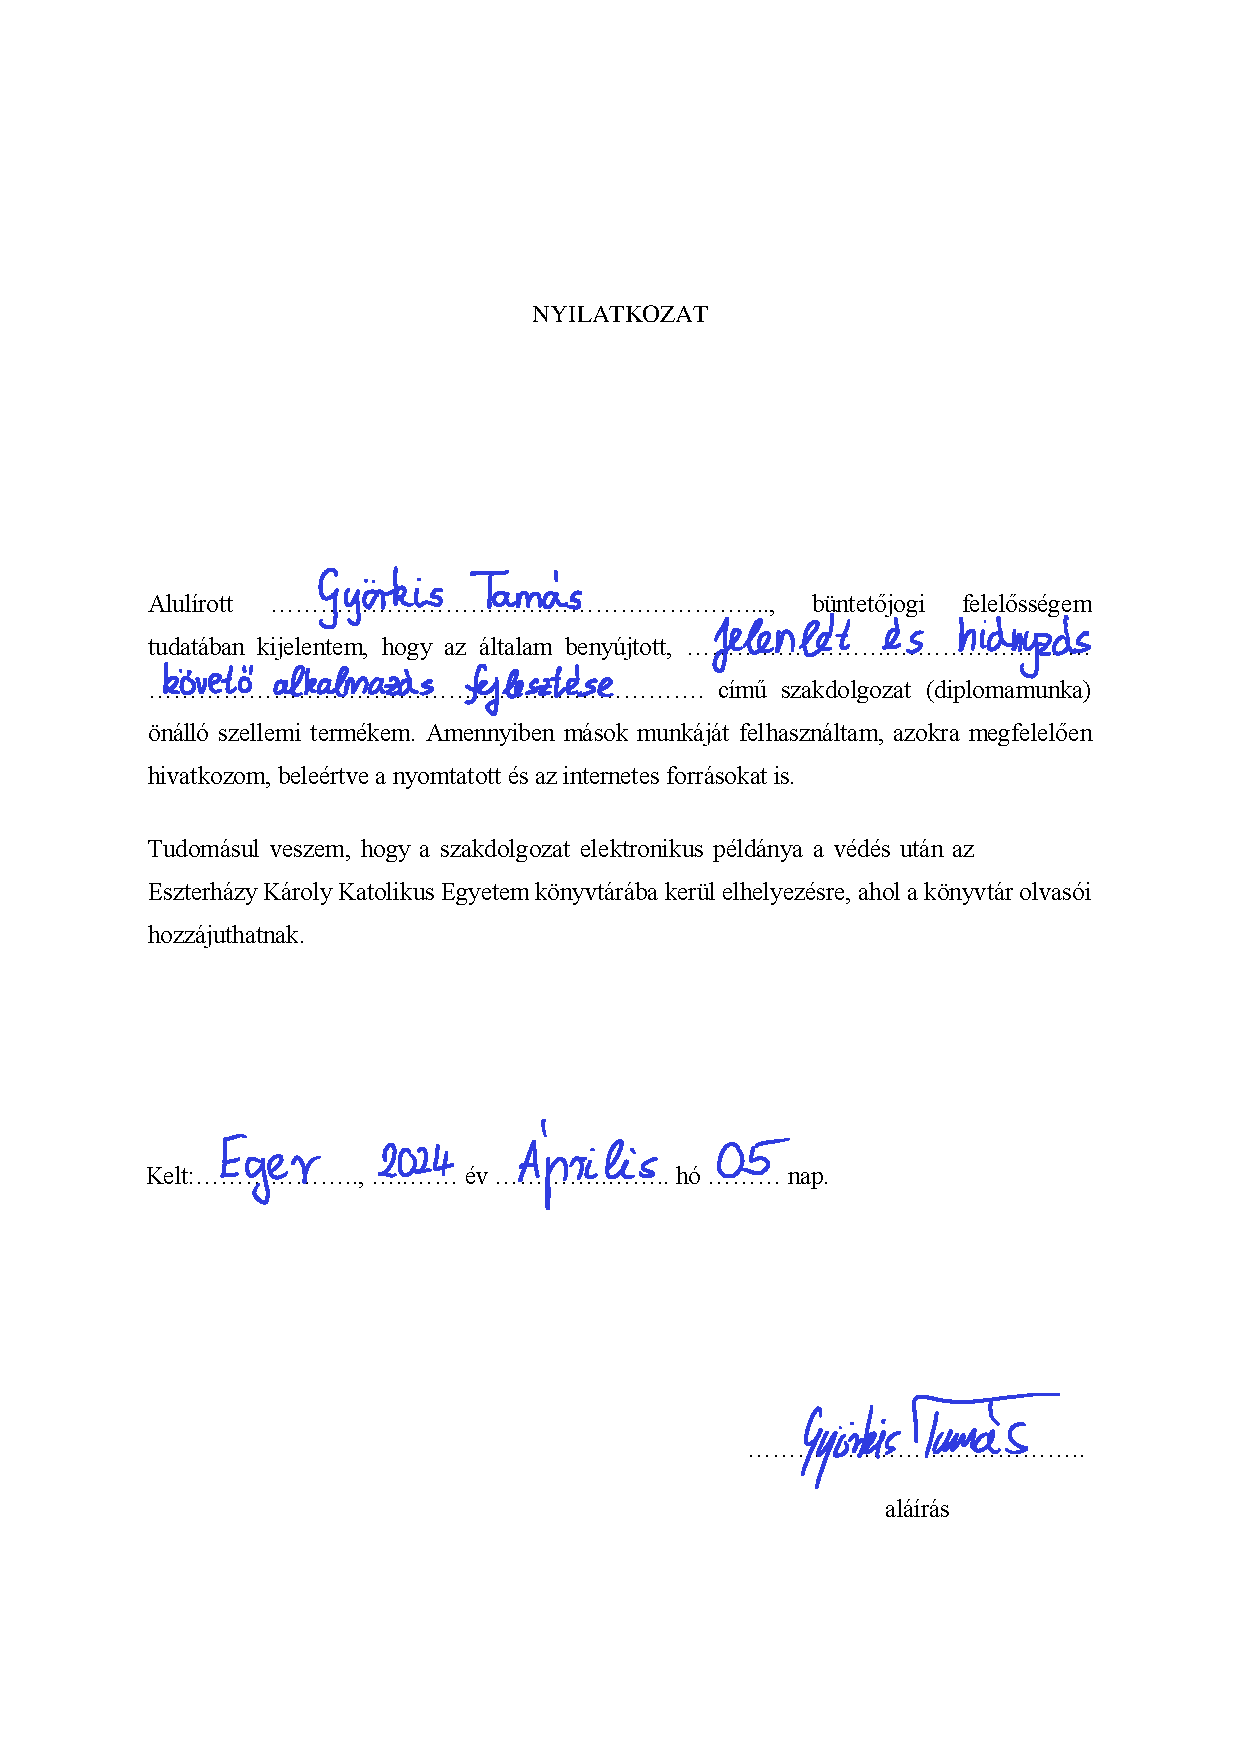
\includepdf{nyilatkozat.pdf}
\end{document}